The maximum required  output  power  of  our  device  was  roughly  calulated as
$\SI{24}{\volt} \cdot \SI{3}{\ampere} = \SI{72}{\watt}$.  Assuming an efficiency
of $\eta\approx \SI{90}{\percent}$ an \SI{80}{W} power supply is required.

The design and construction of a  custom  power  supply  would have consumed too
much  time and resources. Instead, we opted for an external power  supply  which
can be mounted inside the  housing.  The  selected  power  supply  is capable of
supplying  \SI{28}{\volt}  at   \SI{75}{\watt}   and   can  be  seen  in  figure
\ref{fig:circuit:mains-input}.

\begin{figure}[th!]
    \center
    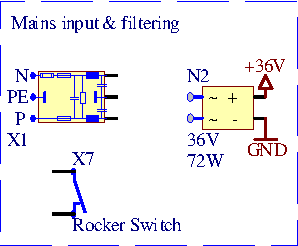
\includegraphics[width=.35\textwidth]{images/circuit/mains-input.pdf}
    \caption{Netzspannung wird gefiltert und auf 36V DC durch ein externes Netzmodul transformiert}
    \label{fig:circuit:mains-input}
\end{figure}

The  device  can be plugged into a power outlet by means of  an  IEC  60320  C13
socket, as illustrated in figure \ref{fig:circuit:iec60320c13}. The socket has a
built-in  fuse  as  well  as  a  built-in  mains  filter, which will reduce high
frequency coupling from the device back into the mains. A rocker switch  is  connected in series with
the socket and the power supply,  allowing  for the end user to cut power at any
time.

\begin{wrapfigure}{r}{.4\textwidth}
    \center
    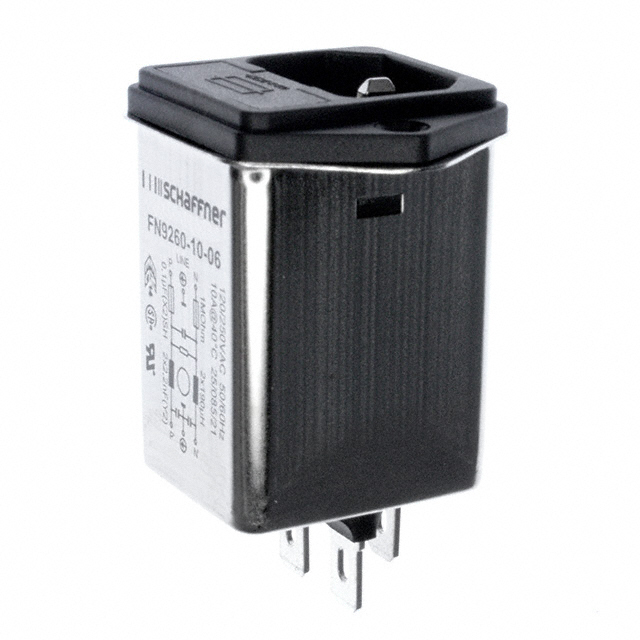
\includegraphics[width=.2\textwidth]{images/circuit/power-entry-module.JPG}
    \caption{IEC 60320 C13 power socket used in this device}
    \label{fig:circuit:iec60320c13}
\end{wrapfigure}

Weiter  wird  eine  Netzeingangs-Steckverbinder  mit integriertem Netzfilter und
Sicherung  verwendet,  was  in der Abbildung  \ref{fig:circuit:mains-input}  als
$X_1$  zu  sehen  ist. Ein auf der R\"uckseit des Geh\"auses montierter Schalter
$X_7$ erlaubt das Ein- und Ausschalten des Endproduktes.

